%!TEX root = ../template.tex
%%%%%%%%%%%%%%%%%%%%%%%%%%%%%%%%%%%%%%%%%%%%%%%%%%%%%%%%%%%%%%%%%%%%
%% appendix4.tex
%% NOVA thesis document file
%%
%% Chapter with Gazebo Setup
%%%%%%%%%%%%%%%%%%%%%%%%%%%%%%%%%%%%%%%%%%%%%%%%%%%%%%%%%%%%%%%%%%%%
\chapter{System Setup on Gazebo Simulator}
\label{app:gazebo_setup}

\section{Introduction}
\label{sec:gazebo_setup_introduction}

Gazebo is a robotics simulator created in 2002 at the University of Southern California. It evolved into a powerful simulator with a large user community around it.

Some of its features are: dynamics simulation with support to various physics engines; advanced 3D graphics using the OGRE rendering engine; it supports many types of sensors and can generate sensor data and noise; it comes with many robot models out-of-the-box; supports tcp/ip communication for remote server simulations; it has a platform for cloud simulation; it supports command-line tools; and it allows for plugin development to extend the functionality.

Gazebo is prepared to interact with \gls{ros} for robot development, via some \gls{ros} packages compiled on the meta-package \textit{gazebo\_ros\_pkgs}.

% section gazebo_setup_introduction

\section{Environment Setup}
\label{sec:gazebo_setup_environment}

The simulation environment consists on a virtual patient room (Fig. \ref{fig:simulation_gazebo_environment}). In it, a patient is lying on bed and the robotic arm lies by the bed side. The room setup tries to replicate a normal patient room with some common hospital apparel.

To create this environment, a set of models were used. The room walls was created directly on Gazebo using its model builder. The other models were obtained from 3D model collection websites. To unite everything, a Gazebo world plugin was created that instantiates all the models. This plugin is loaded via a Simulation Description Format (SDF) file that defines the main Gazebo environment. These files and models all belong to the \textit{smalldrop\_robot\_arm} package.

\begin{figure}[htbp]
	\centering
	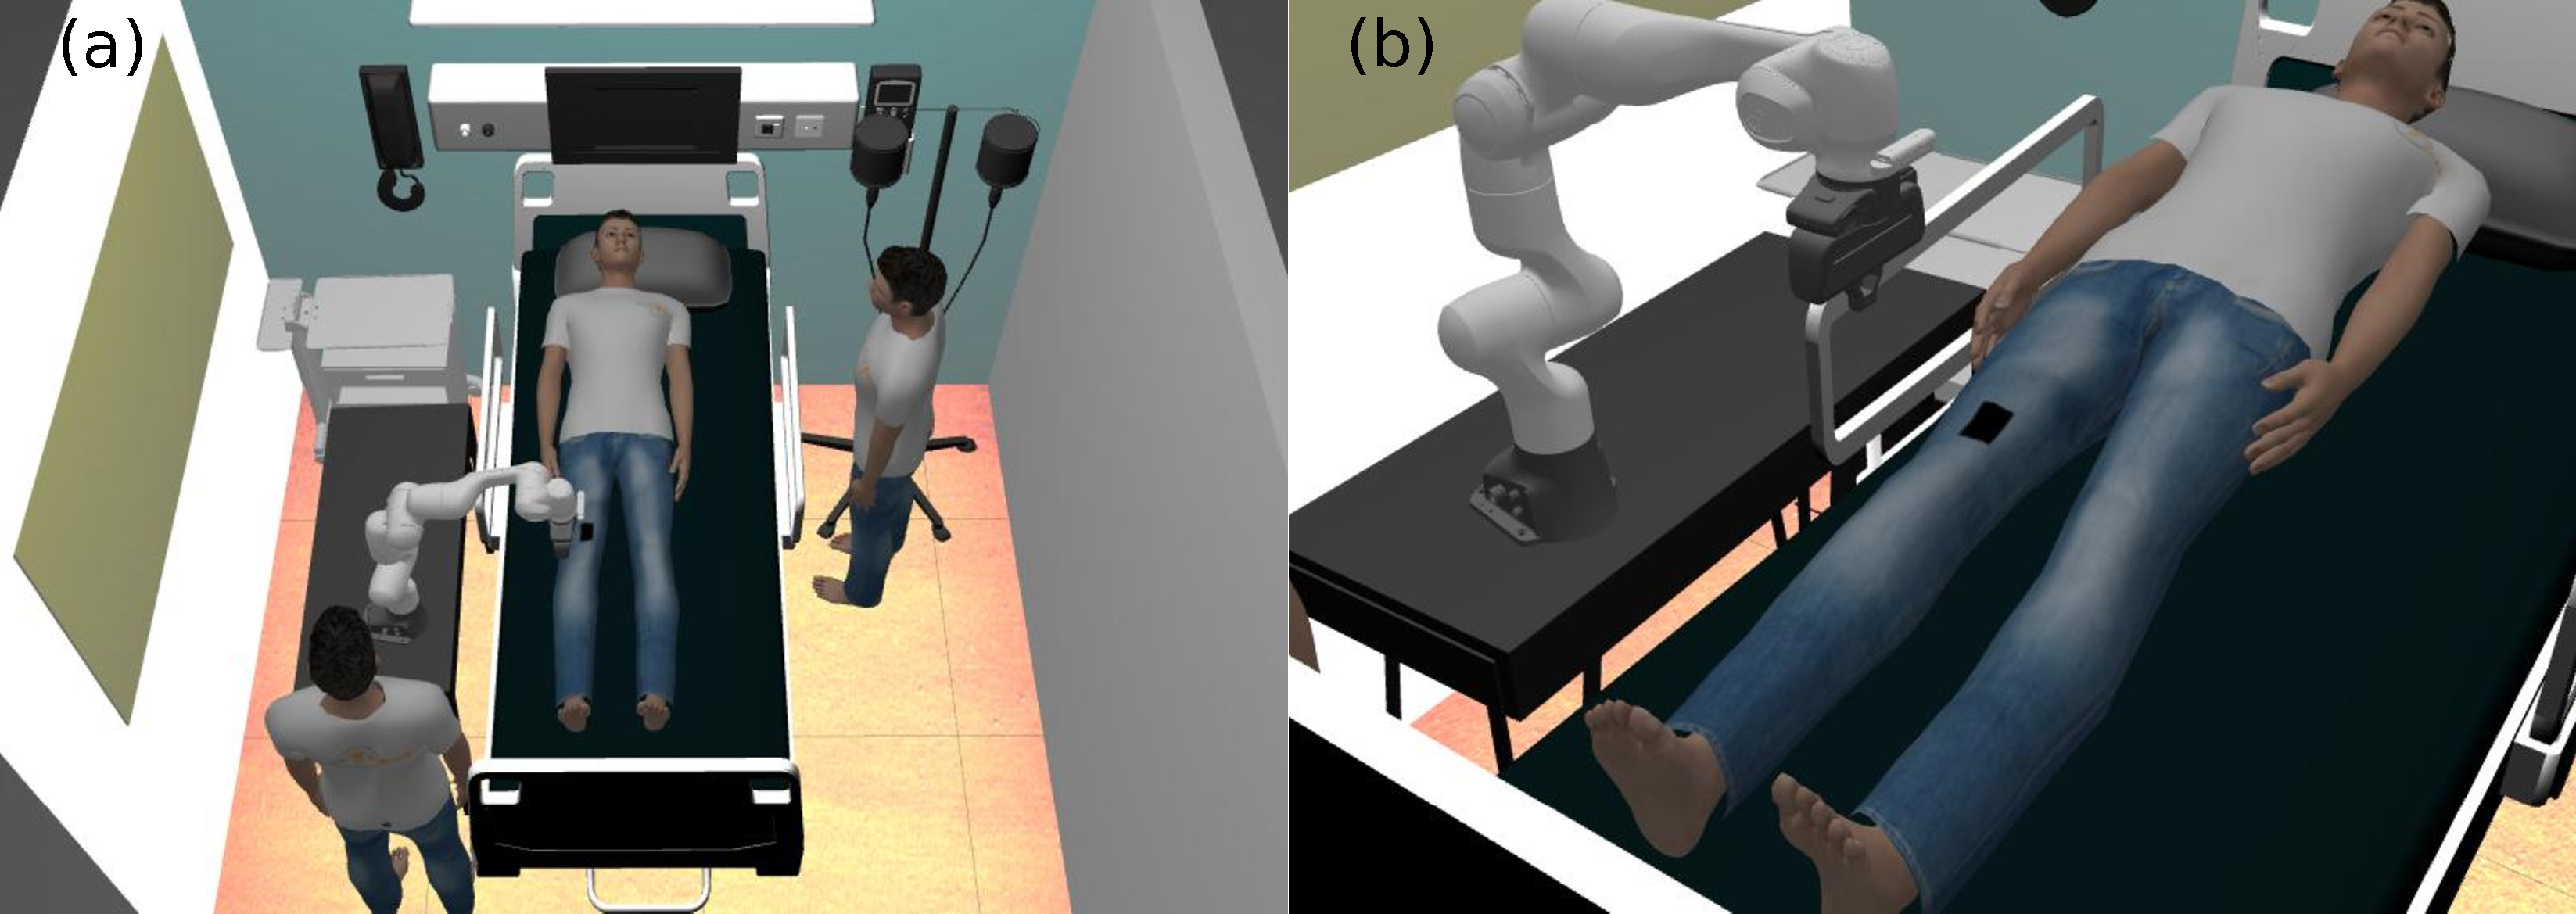
\includegraphics[width=\textwidth]{system_validation_simulation_gazebo_environment}
	\caption[Simulated environment on Gazebo Simulator.]{Simulated environment on Gazebo Simulator. (a) Top-view of the patient room. Gives an overall view of the room's apparel organisation. The standing human models represent clinicians. (b) Close-up on robot and patient.}
	\label{fig:simulation_gazebo_environment}
\end{figure}

% section gazebo_setup_environment

\section{Robot Setup}
\label{sec:gazebo_setup_robot}

In order to simulate the Panda robotic arm on Gazebo, the robot description files need to be updated, and new files added. The original robot description files supplied on \textit{franka\_ros} only describe the robot joints and links basic properties. To do proper physics simulation more data regarding joint transmissions must be added. Two new files were added:

\begin{itemize}
    \item panda.transmission.xacro
    \item panda.gazebo.xacro
    \item panda\_arm.xacro (updated)
\end{itemize}

The first file is where the transmissions are added to each joint. The sintax for transmission configuration is:

\begin{verbatim}
    <transmission name="${robot_name}_tran_n">
        <type>transmission_interface/SimpleTransmission</type>
        <joint name="${robot_name}_jointn">
            <hardwareInterface>hardware_interface/EffortJointInterface</hardwareInterface>
        </joint>
        <actuator name="${robot_name}_motor_n">
            <hardwareInterface>hardware_interface/EffortJointInterface</hardwareInterface>
            <mechanicalReduction>1</mechanicalReduction>
        </actuator>
    </transmission>
\end{verbatim}

On this file, the gazebo\_ros\_control plugin is instantiated. This plugin is responsible for using this info for robot movement control simulation.

The second file is used to configure the color and material of each robot link. The third file is the original robot description file for the robot arm. In this file we update the dynamic properties of the joints like friction and damping.

An online tutorial was followed to do all this setup: \textbf{Integrating FRANKA EMIKA Panda robot into Gazebo} at \url{https://erdalpekel.de/?p=55}.

All these changes belong to the \textit{smalldrop\_robot\_arm} package.

% section gazebo_setup_robot

\section{Camera Setup}
\label{sec:gazebo_setup_camera}

To simulate the camera it was also necessary to update the description files and add a plugin to simulate the image data.

The \textit{realsense2\_description} package contains the description for the camera. In order to simulate the image data, the \textit{realsense\_gazebo\_plugin} was used. The plugin captures the data from the Gazebo environment and publishes via \gls{ros} topics so that it can be used by other packages.

On the package \textit{smalldrop\_vision} the camera description is updated to configure the various data streams. For each stream, things like field-of-view, resolution, clipping and data noise are configured.

% section gazebo_setup_camera